\documentclass{article}
\usepackage{url}
\usepackage{version}

\usepackage{graphicx}


\title{A new DSL for IoT Sychnronisation}
\author{Quanrui MU}

\begin{document}
\maketitle

\begin{abstract}
We rely here on model driven engineering to propose a new DSL for IoT. Our case study applies for health car systems and particularly we consider signal synchronisation\footnote{\url{https://blog.endaq.com/synchronizing-signals}} between both EEG and ECG devices.  Our main goal to ensure the transformation from the model into formal language such as Signal and/or LOTOS in order to rigorously check needed properties. 
\end{abstract}

\textbf{Keywords:} IoT, MDE, Hybrid Systems, Signal Synchronisation, Distributed System Composition, Cyber Physical Systems. 

\section{Introduction}

\paragraph{}

In multi-system signal transmission, the synchronization has always been a problem that needs to be solved, especially for IoT devices. In order to obtain data describing a state in a specific and accurate time, the signal receiver must synchronize the signals from different devices depending on the clock, otherwise the output signal has a phase gap on the clock, which will cause incorrect judgments when multiple data are used. 

The main problem to be solved in this project is the synchronization of data output signals for IoT devices, especially medical devices such as ECG and EEG devices when they are used at the same time. Using the method of model-driven engineering, we design the meta-model for the data acquisition, processing and output of the IoT devices, and according to the specific requirement of ECG and EEG signal synchronization, we instantiate the model for this specific problem, and complete the model conversion in order to generate the Java project that can complete the corresponding function.

\section{IoT Definition:} 

\paragraph{}

The Internet of Things (IoT) refers to a network that enables Internet-connected objects to use embedded sensors for data collection and exchange. And the IoT device is any independent Internet-connected device that can be monitored or controlled from a remote location. The essence of the IoT is still the Internet, but the terminal is no longer a computer (PC, server), but an embedded computer system and its supporting sensors. This is the inevitable result of the development of computer technology. Computers serving humans take on various forms, such as wearable devices, environmental monitoring devices, virtual reality devices, and so on. As long as there are hardware or products connected to the Internet and data interaction occurs, it is called the Internet of Things.

\section{Application Domains}

\begin{itemize}
	\item Autonomous cars
	\item Telecommunication : ESim
	\item Health care  : EEG and ECG
	\item Edge Computing 
\end{itemize}

In our case, we consider healthcare case study. 

\section{State-of-the-Art}

\paragraph{General understanding of ECG signals} 

\paragraph{}

Electrocardiography is a graph of voltage versus time of the electrical activity of the heart using electrodes placed on the skin\cite{ref1}. These electrodes detect the small electrical changes that are a consequence of cardiac muscle depolarization followed by repolarization during each cardiac cycle (heartbeat). 

There are 3 main components to an ECG:

\begin{enumerate}
  \item the P wave, which represents the depolarization of the atria; 
  \item the QRS complex, which represents the depolarization of the ventricles; 
  \item and the T wave, which represents the repolarization of the ventricles.
\end{enumerate}

\begin{figure}[htbp] 
\centering 
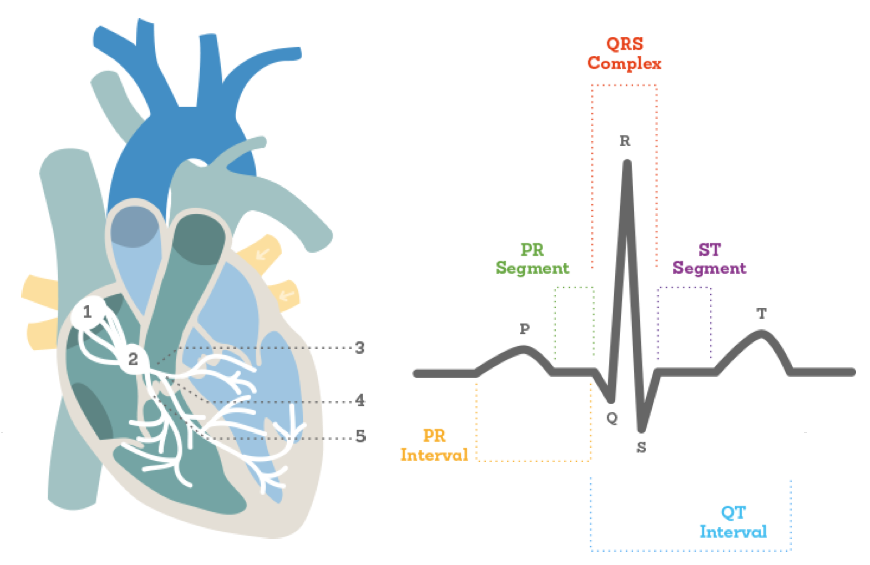
\includegraphics[width=0.8\textwidth]{ECG.png} 
\caption{ECG Wave Pattern} 
\label{Fig.main1} 
\end{figure}

\paragraph{General understanding of EEG signals} 

\paragraph{}

Electroencephalography (EEG) is an electrophysiological monitoring method to record electrical activity on the scalp that has been shown to represent the macroscopic activity of the surface layer of the brain underneath\cite{ref2}.

The EEG is typically described in terms of (1) rhythmic activity and (2) transients. The rhythmic activity is divided into bands by frequency. According to different frequencies, EEG waveforms are divided into Delta, Theta, Alpha, Beta, Gamma, Mu.

\paragraph{Formalizing Electrocardiogram (ECG) Signal Behavior in Event-B} 

\paragraph{}

In this paper a method is proposed to formalize and validate the specifications of ECG signals in Event-B. They formally define the waves of ECG and their relation, and then formalize and validate several properties about their behavior.

There are three phases through which the heart produces the ECG, the first is the activation of the atria, during which a wave called P wave is generated by the sinoatrial node (SA)\cite{ref3}. The second is the activation of the ventricles, during which a wave called QRS is generated by the atrioventricular node (AV). Finally, the recovery phase during which a wave called T wave is generated throughout the heart muscles recovery phase. In addition, there are flat signals that represents no activity between these two waves for certain periods of time. These inactive periods are represented as flat segments between the above waves. The frequency of occurrence of these waves, their duration, and their existence reflects several facts about the heart behavior such as normal, fast, slow, or abnormal status.

From this paper and the above general understanding, we can know that the waveform pattern of ECG is established and regular, so the signal obtained is continuous and meaningful.

\paragraph{Window Functions Analysis in Filters for EEG Movement Intention Signals} 

\paragraph{}

The window functions are commonly used in different digital signal processing (DSP) applications as signal preprocessing (denoising), analysis and estimation signal, digital filter design and speech processing.

The work in this paper is to find the adequate window function that enhance the movement intention signals in electroencephalography (EEG)\cite{ref4}. The electroencephalogram (EEG) records the brain electric activity, usually described in five frequency oscillations known as brainwaves: delta (0.5–4Hz), theta (4–8 Hz), alpha (8–13 Hz), beta (13–30 Hz), and Gamma (30–128 Hz). There is also the Mu (μ) rhythm that it is a sub-band of alpha (9–11 Hz) [10], this rhythm is directly related with the movement. 

The EEG presents some characteristics such as the non-periodicity, non-standardized patterns, and small voltage amplitudes. These attributes lead to the EEG signal to be easily mixed up with noise, making it harder to recognize and extract meaningful information from the EEG signals, particularly electrophysiological information. 

From this paper and the above general understanding, We can understand that although the EEG signal is continuous from the perspective of the sensor, for actual medical observations, only meaningful signal data during brain activity is needed, that is, the signal data will be extracted on top of the basic signals, we have to perform a filtering to obtain discrete and meaningful signals.

\paragraph{Design of a domain specific language and IDE for Internet of things applications} 

\paragraph{}

The development of IoT application design environment based on the high level visual programming language in form of Editor within the class of visual domain specific modeling languages (VDSML) using formal presentations and abstract syntax, has been presented in this paper. The front end of the Editor is based on JavaScript language\cite{ref5}.

The development dilemma of IoT applications is: 

\begin{itemize}
  \item heterogeneity; 
  \item specifics.
\end{itemize}

That is, wide range of hardware and software entities running on specific platforms, middleware specific features, which can be solved by integrated development environment (IDE) based on domain specific high level language:

\begin{itemize}
  \item abstract most of these intricacies and specifics in hardware, software, communication media and protocols; 
  \item the language should be capable to support large scale design of these systems by combining several design blocks and saving them in application libraries, importing them, reconfiguring and parameter setting with ease for new tags and locations, enabling reusability and scalability.
\end{itemize}

\paragraph{A Methodology Based on Model-Driven Engineering for IoT Application Development} 

\paragraph{}

In this paper, a methodology based on Model-Driven Engineering with different levels of abstraction is proposed, including points of view, and granularity, with the objective of guiding the development of software applications for Internet of Things. The methodology is supported by methods of model transformation, enabling the generation of the code of the software applications for Internet of Things\cite{ref6}. In addition, a Service-Oriented Architecture is presented for the deployment of software applications, composed of four layers that allow the identification of the components required for the implementation of the Internet of Things systems.

\begin{enumerate}
  \item Object Layer: composed of hardware objects available on the network that detect the state of things; 
  \item Network Layer: consists of the infrastructure that supports wired, wireless or mobile connections between things, allowing to detect their environment, which enables to share data between connected things, enabling event management and intelligent IoT processing; 
  \item Service Layer: there are created and managed the services required by the users or software applications, the service layer is based on middleware technologies, which is fundamental for consuming services and the execution of IoT applications, where hardware and software platforms can be re-usable;
  \item Application Layer: responsible for delivering the applications to different IoT users.
\end{enumerate}

\paragraph{A Hybrid Approach for Synchronizing Clocks in Distributed Systems} 

\paragraph{}

Clock synchronization in a distributed system can be referred to clock recovery which is achieved by frequent synchronization in serial communication. In this paper they have implemented a hybrid method for synchronizing clocks in a distributed system which achieved better synchronization accuracy than the traditional NTP synchronization\cite{ref7}. 

\paragraph{The Signal Synchronous Multiclock Approach to the Design of Distributed Embedded System} 

\paragraph{}

In this paper, there is a synchronous model for design and validation. This model offers an adequate formal basis to deal with the reliable design of embedded systems\cite{ref8}. Its basic assumption is that computation and communications are instantaneous from the point of view of a logical time, referred to as "synchrony hypothesis". 

A fully synchronous system is characterized by the boundness and knowledge of: i) processing speed, ii) message delivery delay, iii) local clock rate drift, iv) load pattern, and v) difference among local clocks. A fully asynchronous system assumes none of these characteristics.

The central question is not to agree on a global time, but to agree on the common event occurrences during the interaction of components. Compared to the synchrony/asynchrony definition, the polychronous model offers an intermediate vision: while it assumes the boundness of computation and communication activities, the difference among local activation clocks is a priori unknown.

The polychronous system consists of two concurrent sub-systems that receive control from events a and b and conditionally communicate via an event c or do something else (d or e). It can be refined into a single-clocked system, by synchronizing the events a and b. It can be also refined into a distributed system, by distributing a and b on two different locations and by implementing c by a FIFO communication channel. In general, the reliability of such channels is implicitly assumed in the polychronous model. However, in this paper, it is explicitly proved.

\begin{figure}[htbp] 
\centering 
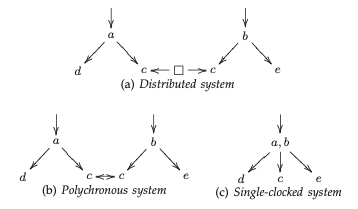
\includegraphics[width=0.8\textwidth]{DistributedSystem.png} 
\caption{Distributed,polychronous and single-clocked systems} 
\label{Fig.main2} 
\end{figure}

In this paper there is a method to design entirely distributed embedded systems with a synchronous language by proposing a general methodology composed of four steps detailed in the following chronological order:

\begin{enumerate}
  \item System specification and manual distribution: modeling of application functionality, distributed hardware architecture, and their association; 
  \item Automatic transformations: guaranteeing the global functional correctness of the distribution;
  \item Deployment on specific platforms: instantiating the parts of the resulting model with components that represent specific platform mechanisms, e.g. for communication, synchronization;
  \item Non function analysis and automatic code generation:checking the non functional (temporal) constraints induced by the chosen deployment and distributed code generation.
\end{enumerate}

\paragraph{Development of Real-Time ECG Signal Monitoring System for Telemedicine Application} 

\paragraph{}

This work presents the development of low cost, portable real-time Electrocardiogram (ECG) signal monitoring system with abnormality detection capability. The architecture of this application is of great reference for our project, because it implements the whole process framework from sensor signal acquisition and transmission, communication mechanism to receiving end display and analysis.

In this paper, the real time ECG signal monitoring system is proposed to address the above issues\cite{ref9}. The heart rate is calculated and any abnormality in the heart rate is intimated to doctor through GSM module. Further, the duration of different ECG signals is extracted from ECG waveform and displayed in PC which can be accessed by the doctor through remote login procedure when he gets an SMS alert on his mobile phone. Our project does not have the following analysis and reminder functions, but this method of connection communication can be used. Another big difference is that we need to implement different input devices, not just one device.

\section{Design for the meta-model}

\paragraph{Meta-model establishment for signal synchronization of IoT devices} 

\paragraph{}

\begin{figure}[htbp] 
\centering 
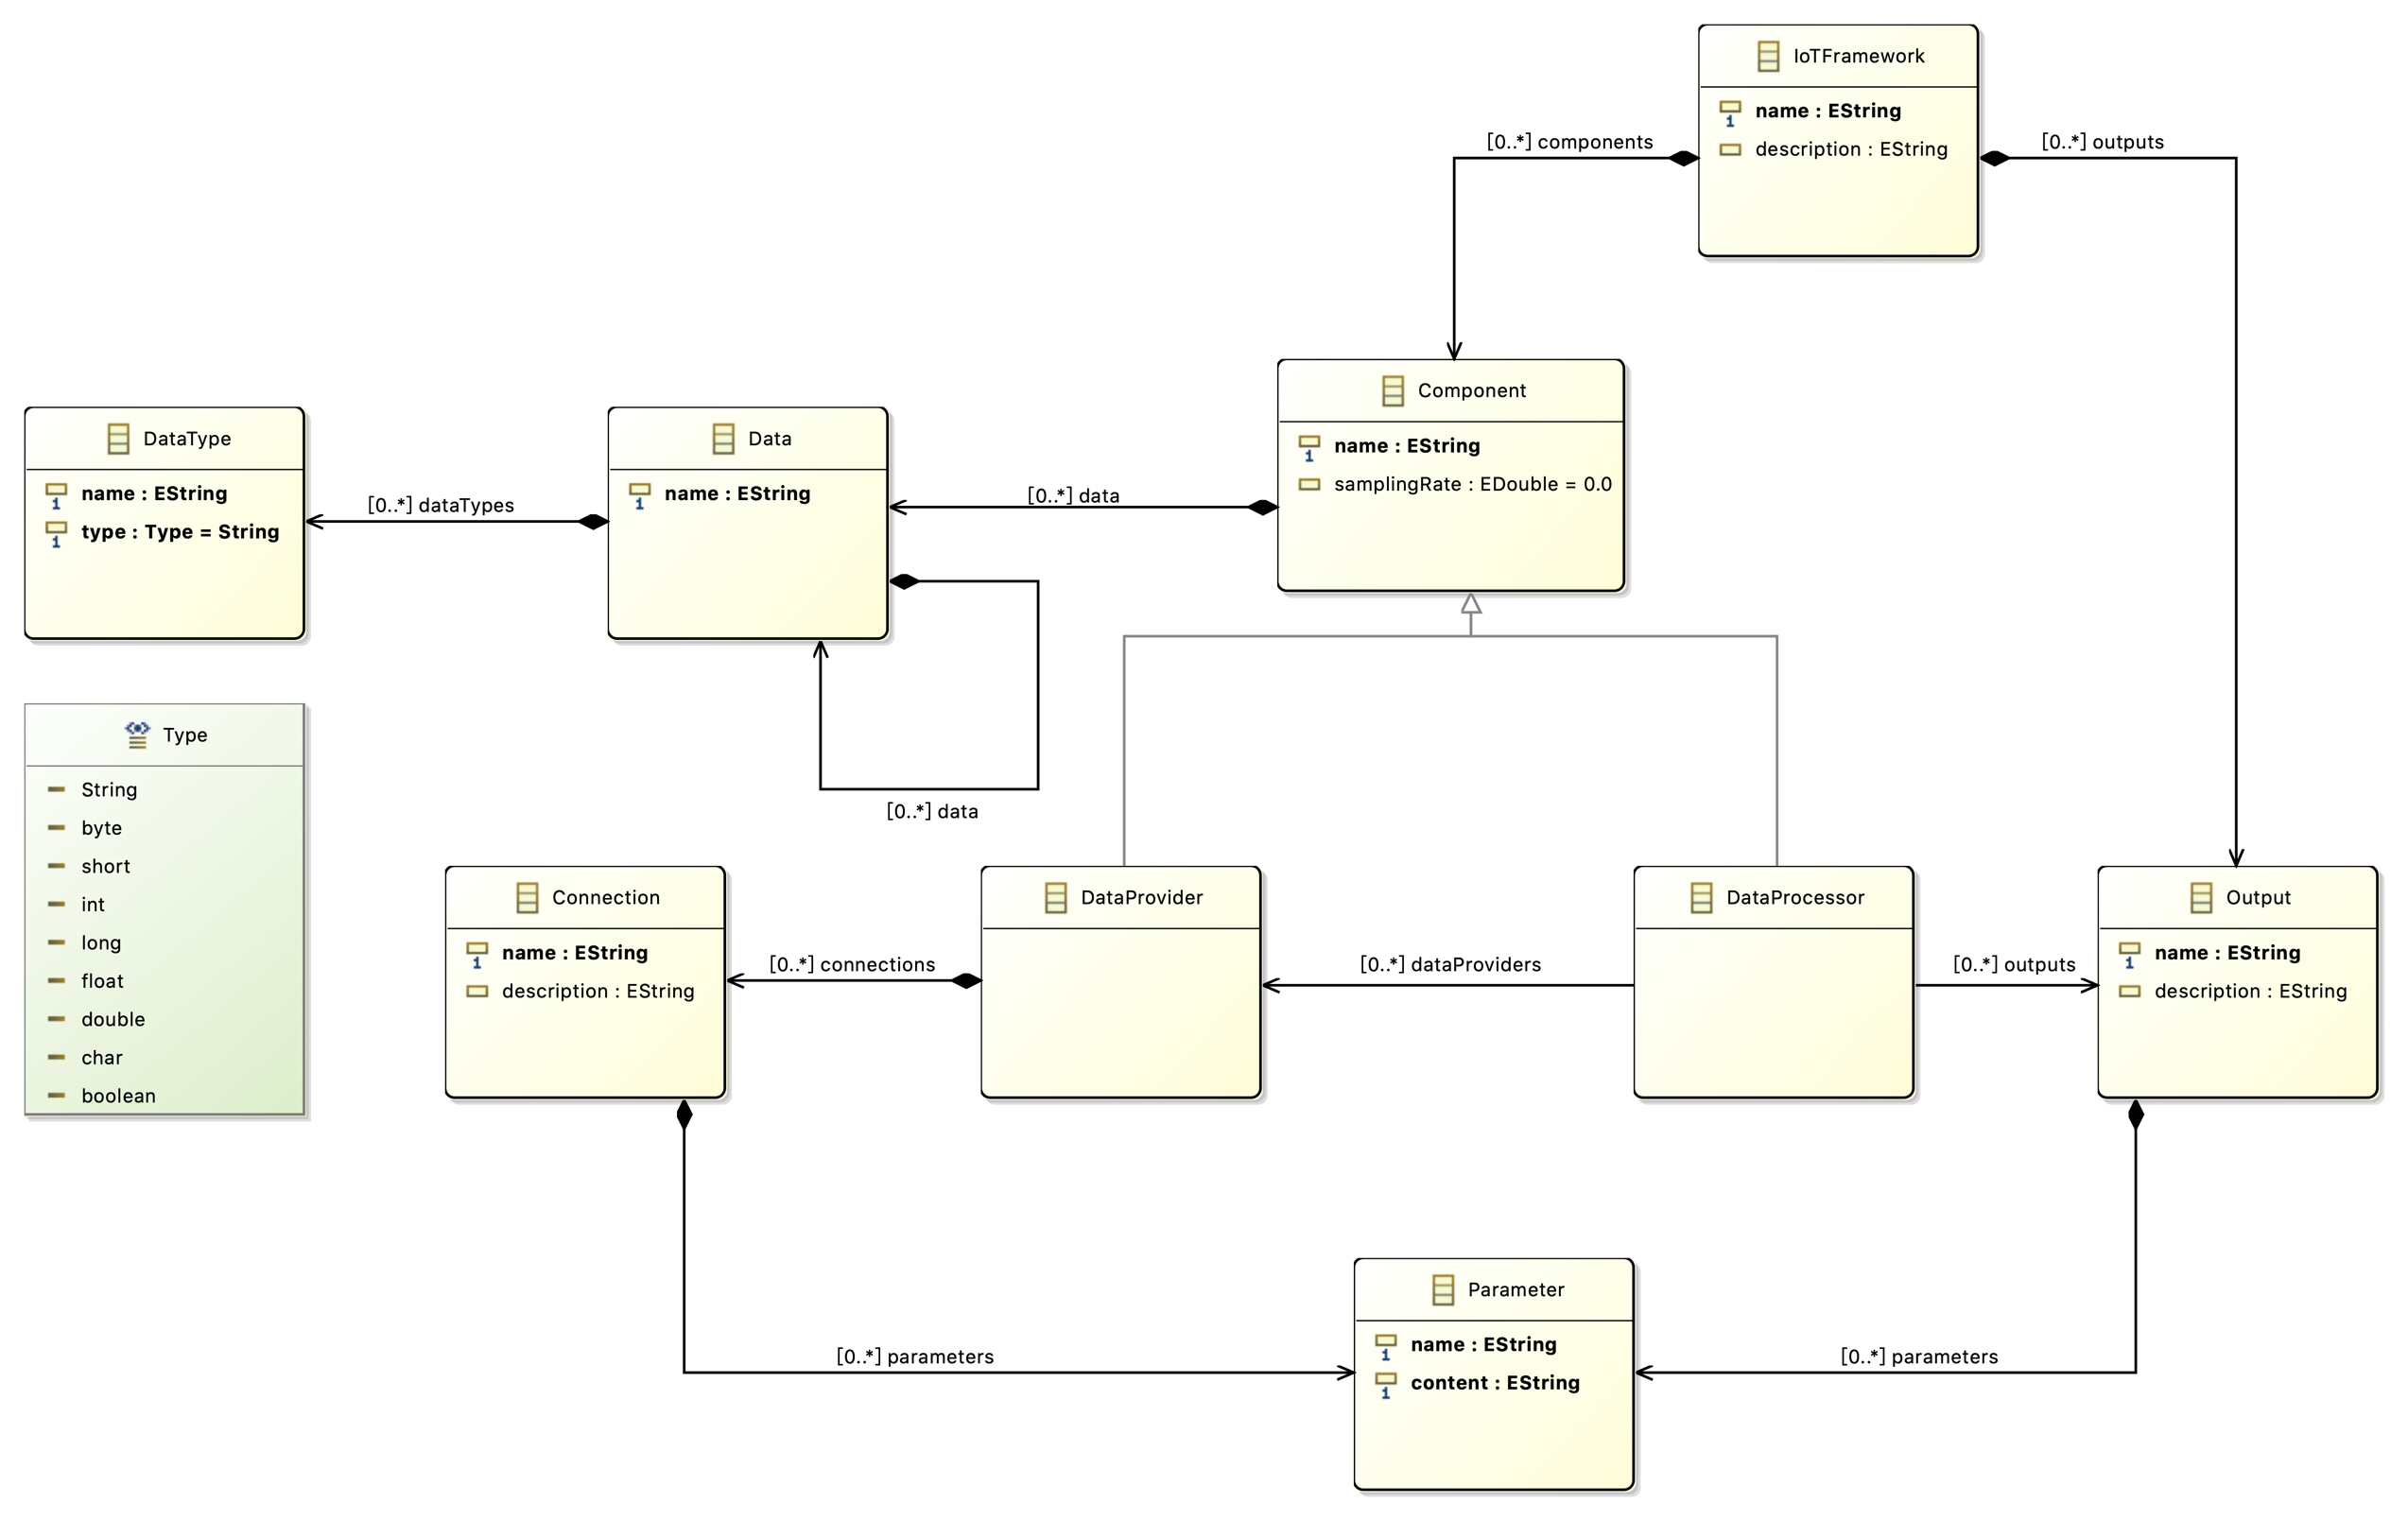
\includegraphics[width=0.8\textwidth]{IoT class diagram.jpg} 
\caption{IoT Framework meta-model} 
\label{Fig.main3} 
\end{figure}

\begin{itemize}
  \item IoTFramework: The first layer of the meta-model, the foundation of building the model is to build an IoTFramework as a root.
  \item Component:  the component part of the model. The main attributes are name and samplingRate, which are the basic attributes of the device and the processor.
  \item DataProvider: the device that provides the data, a subclass of the component.
  \item DataProcessor: component that process signals obtained by different devices, also subclass of component.
  \item Output: the part where the processed data is output and displayed can be modeled as a console, monitor, or database.
  \item Connection: used by DataProvider, responsible for providing parameters and information for device connection.
  \item Parameter: as a component of connection and output, it can be modeled as multiple parameters to describe information.
  \item Data: for different DataProvider and DataProcessor, different formats of data are required to describe the signal, so Data is a part of the Component and describes the data format which we use.
  \item DataType: Data is composed of DataType, which can be modeled as multiple classes with different data names and data types to form different data.
\end{itemize}

\paragraph{The OCL establishment for the specific constraints of the meta-model} 

\paragraph{}

\begin{itemize}

    \item IoTFramework, Component, Output name specification: not empty, greater than 2 characters, starting with a letter, consisting of letters and numbers.
    \item DataProvider: samplingRate must be greater than 0.
    \item DataProcessor: If the output is not 0, dataProviders is not 0. SamplingRate must be between the maximum and minimum of dataProviders. The DataProvider of the DataProcessor must have at least one Connection. Each DataProvider for this DataProcessor must have at least one Data. Each DataProvider for this DataProcessor must have at least one Data.
    \item Data: Data must have at least one DataType or at least one Data with DataType. Data can not have two DataTypes which are exactly the same. And the Data can not have two-level nesting.
    \item Parameter: Connection and Output cannot have two parameters with the same name.

\end{itemize}

\paragraph{The Xtext establishment for the syntax description of the meta-model} 

\paragraph{}

Using the Xtext plug-in provided by EMF, we can create a domain specific language description for this meta-model, and the generated syntax can be deployed to the Eclipse plug-in environment so that we can use this new syntax to create a textual model that is more specific, easier to describe, and more intuitive. We adopt a syntax similar to XML, which also makes it easier for users to get start to it.

\section{Design for the model}

\paragraph{Model establishment for signal synchronization of ECG and EEG devices} 

\paragraph{}

\begin{figure}[htbp] 
\centering 
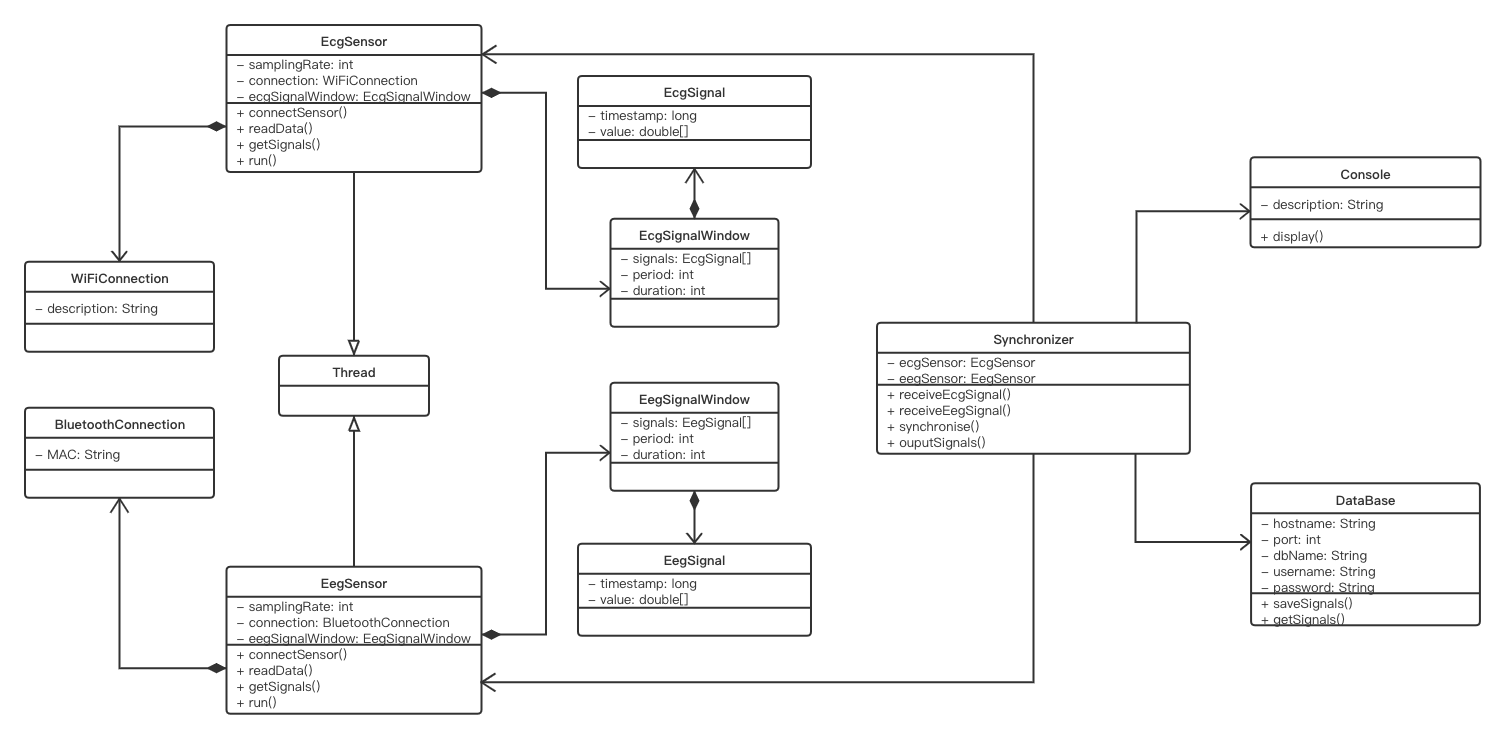
\includegraphics[width=0.8\textwidth]{Sync signal 5.3.png} 
\caption{Sync Signal UML Model} 
\label{Fig.main4} 
\end{figure}

\begin{itemize}
  \item EcgSensor/EegSensor: instantiated by DataProvider and used as thread class to connect ECG/EEG devices to obtain data.
  \item WiFiConnection/BluetoothConnection: instantiated by Connection and provides a series of parameters for the connection to device. For different connection methods, the required parameters are different, so the attributes are instantiated by Parameter.
  \item EcgSignalWindow/EegSignalWindow: instantiated by Data, is a data entity that encapsulates a series of attributes of the signal provided by the device. Because different devices provide different signal formats, the attributes are instantiated by DataType.
  \item EcgSignal/EegSignal: instantiated by Data, is a data entity that encapsulates the signal value with timestamp, as the signal is an integral part of the signal window, this makes use of the self-composition relationship of Data.
  \item Synchronizer: instantiated by DataProcessor, the central part of the framework for synchronizing ECG and EEG signals, find the first signal time of both devices that match with the local clock, and then output following signals according to the difference between local clock and device clock of both devices.
  \item Console/DataBase: instantiated by Output, is responsible for output and display of the signals after synchronization, like Connection, different methods of output requires different parameters, so those attributes in those classes are instantiated by Parameter.
\end{itemize}

\paragraph{Model generated from meta-model in line with the design for function} 

\paragraph{}

\begin{figure}[htbp] 
\centering 
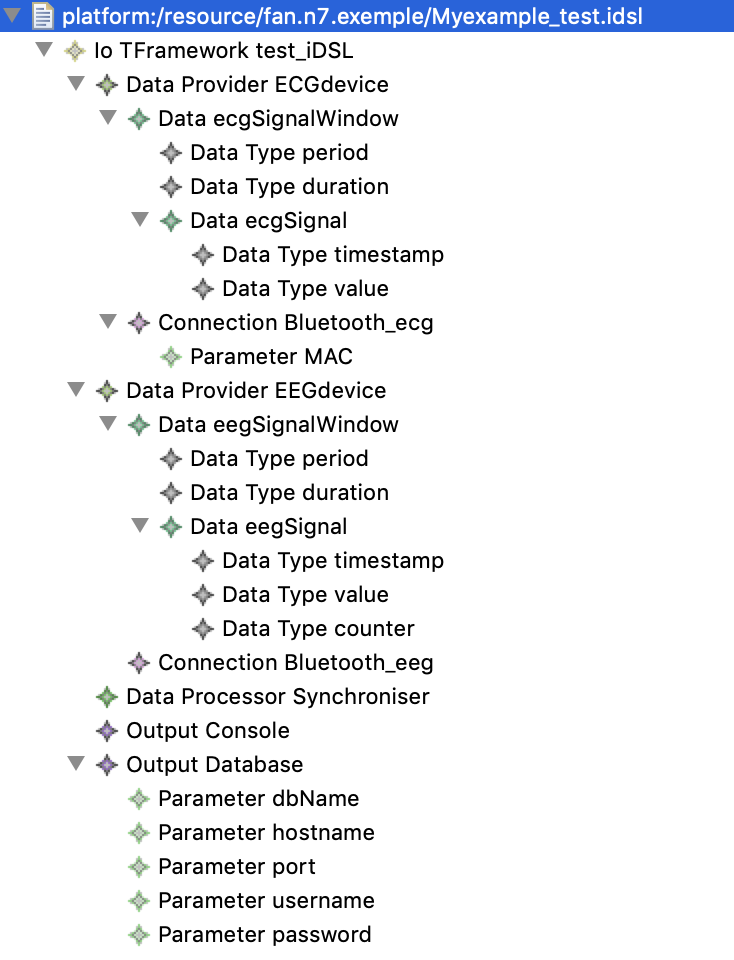
\includegraphics[width=0.8\textwidth]{Model generated from the meta-model.png} 
\caption{Model generated from the meta-model} 
\label{Fig.main5} 
\end{figure}

Using meta-models and EMF tools, we can directly build a model that conforms to our UML design, and use OCL to verify it to meet the constraints which make the model have no errors.

\paragraph{Textual model generated from meta-model using Xtext syntax} 

\paragraph{}

\begin{figure}[htbp] 
\centering 
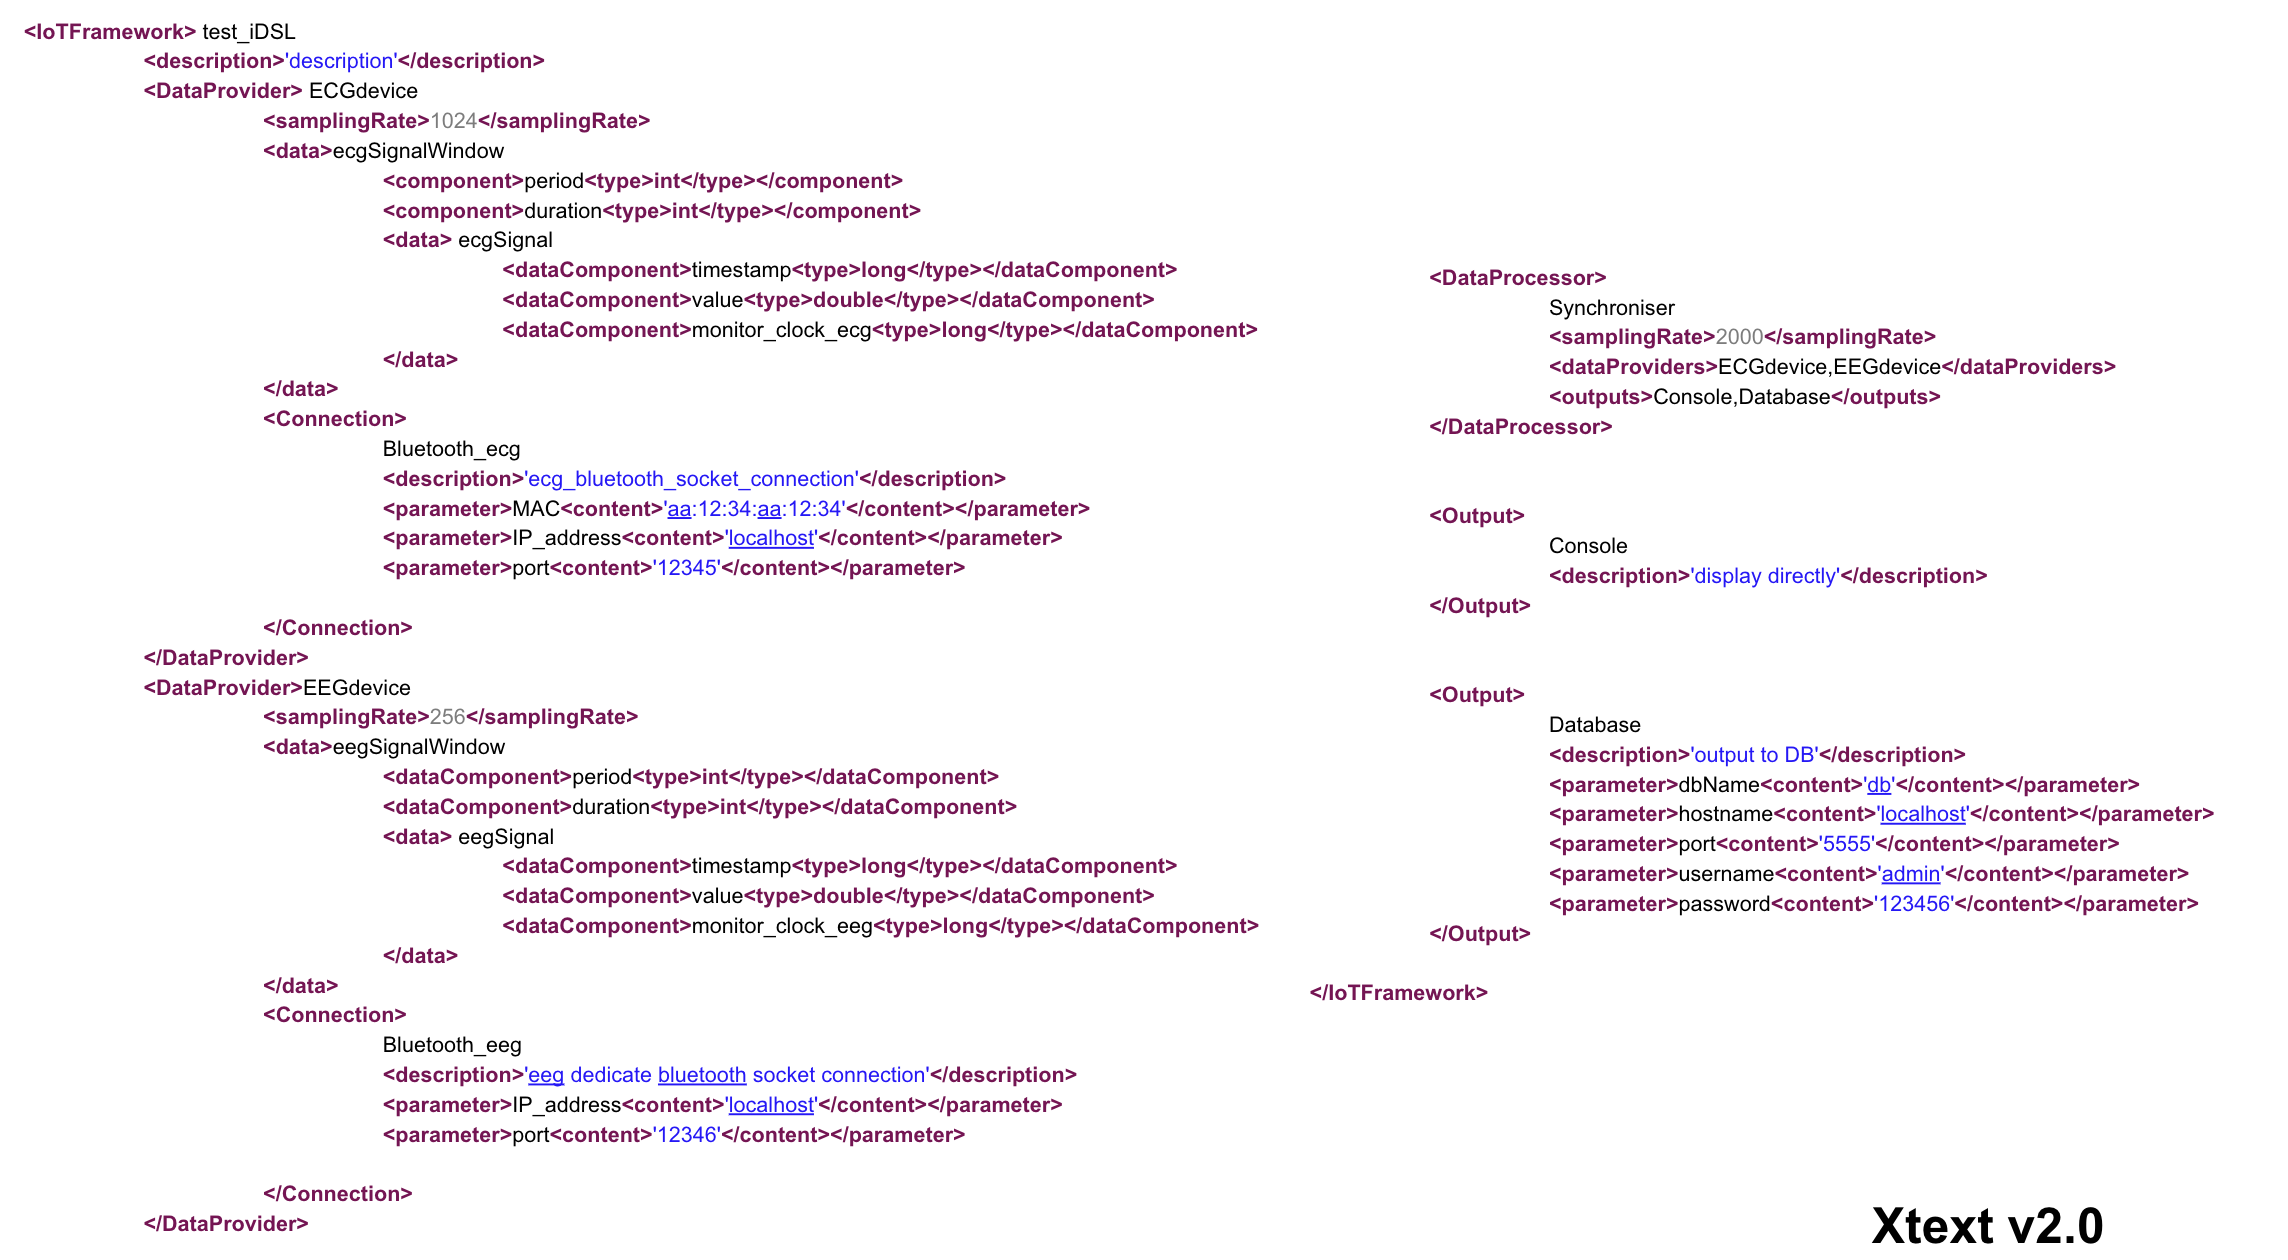
\includegraphics[width=0.8\textwidth]{Xtex textual model.png} 
\caption{Xtext textual model} 
\label{Fig.main5} 
\end{figure}

Using the Xtext syntax similar to the XML format that we defined for the meta-model, the model can also be implemented through textual description.

\paragraph{Textual model generated from meta-model using Xtext syntax} 

\paragraph{}

\begin{figure}[htbp] 
\centering 
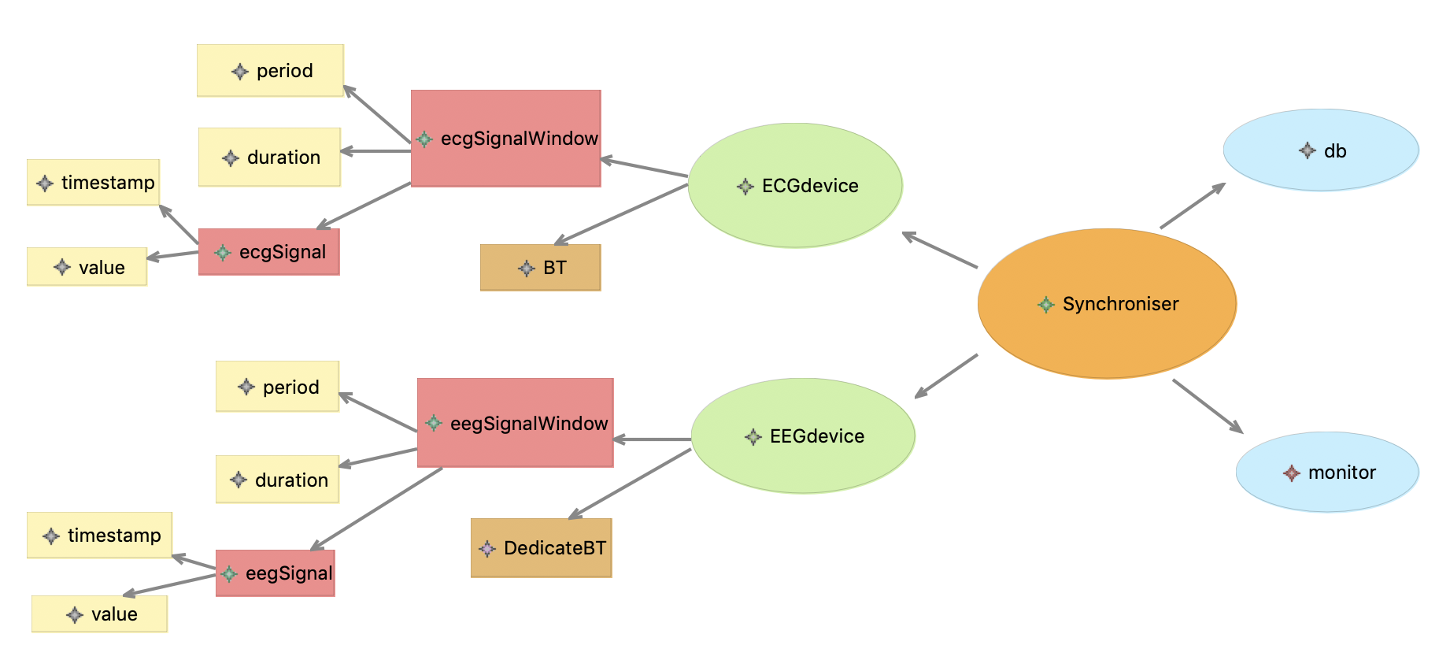
\includegraphics[width=0.8\textwidth]{Graphic presentation of the model with Sirius .png} 
\caption{Graphic presentation of the model with Sirius} 
\label{Fig.main5} 
\end{figure}

Sirius is a tool provided by Eclipse for graphical presentation of models, which can make our model more direct and clear.

\section{Implementation with model transformation}

\paragraph{Model transformation by Acceleo} 

\paragraph{}

Acceleo is an open source code generator for Eclipse that allows us to build applications using a model-driven approach. 

Although our model has been established and has a text description similar to the code, the problem is that we do not have a tool like a compile to execute our model in real computer and realize its corresponding functions. The reason is that we only have the definition and presentation of the model, but there is no way to create a runtime environment for it. Nevertheless, with Acceleo, we can transform the model defined above into executable Java code, and use the Java runtime environment to execute our program and realize those functions.

\paragraph{Synchronization method design}

\paragraph{}

In the executable project, the most important method to be implemented is to synchronize the signal. In our design, the process of synchronizing the signal is mainly divided into three steps: find the head, find the corresponding synchronized signal, and output.

\begin{enumerate}
    \item Find the head: In this system composed of ECG and EEG and signal recerver, there are three clocks, the local clock of ECG, the local clock of EEG, and the local clock of the receiver and it is inevitable that there may be some errors in these three clocks. Since ECG is a discontinuous signal, and EEG is a continuous signal, whenever we receive an ECG signal for the first time, we need to find the corresponding or closest EEG signal that has been received for the first time in the same absolute time, this process is done with the their common reference clock, the receiver’s local clock. By calculating the difference between the timestamp of each signal and the receiver’s local clock when receiving those signals, we can find the first EEG signal.
    \item Find the corresponding synchronized signal: As long as the corresponding first EEG signal is found, we sequentially retain the ECG signals received next, and then search for the corresponding EEG signal according to the sampling rate.
    \item Output: For the synchronized signal found in the second step, we output them in the manner described in the output class, and the result displayed is the synchronized signals.
\end{enumerate}

\paragraph{Java program test}

\paragraph{}

After the execution of Accelo, we can get the Java project transfored from the model. In order to simulate the running process of the entire program, we have established two client programs to simulate the ECG and EEG devices. These two programs create connection and start commucation with the main program called Synchronizer which is transformed from our model through Socket. The main program successfully receives the ECG and EEG signals continuously provided by the two client programs, completes the synchronization, and outputs the synchronized signal data. The result inlustrates that the project successfully achieves the entire process of signal acquisition, synchronization, and output.

\paragraph{Model transformation into SIGNAL}

\paragraph{}

SIGNAL is a programming language based on synchronized data-flow\cite{ref10}. The SIGNAL formal model provides the ability to describe systems with multiple clocks, which exactly meets the requirement of our specific application scenario. Therefore, if we can transform our model to a SIGNAL model, it will be more convenient for description of data input, synchronization and output.

In SIGNAL language, a signal is a sequence of values of the same type, which are present at some instants. The set of instants where a signal is present is the clock of the signal. We can use set of instant to describe the time stamp of the input ECG or EEG signal, and the value of the corresponding position to describe the value of the signal, thus completing the signal input. In the matter of time, events are considered only according to their relative order, which means a value from a signal can occur before a value of another signal, or after, or at the same instant. But after get inputs, The synchronization method can be implemented with the operators in SIGNAL. SIGNAL provides Monochronous operators, Delay operators and all other operations, which can help us to transform the synchronization method into a description in SIGNAL language.

\section{Conclusion}

\paragraph{}

Our research started from the actual applicable situation of displaying synchronized signals when using ECG and EEG devices at the same time. While thinking about how to solve this problem, we tried to generalize and model this process.

The main reason for this problem is the clock synchronization of multiple systems. The timestamp on the signal of each system must be the local clock of the system, but on the receiver side, we need to synchronize the signals from different systems. This is a problem we need to solve for this specific application scenario, so at the very beginning our work focused on designing a method that can synchronize the signals from ECG and EEG equipment. By understanding and learning of state of the art of synchronization methods of discrete and continuous signals, a method for synchronizing ECG and EEG signals at the receiving side was designed.

In order to make the solution process of this problem and many other similar problems in the application scenarios of IoT devices have a standardized solution process, through the idea of model-driven engineering, we tried to abstract and model this process. Therefore, a meta-model for the interaction and processing of IoT devices and data is obtained. With the help of various tools such as Xtext provided by EMF, a graphical description and textual description of this meta-model are designed.

We instantiated the model from our meta-model for this specific scenario according to the application of the ECG and EEG device signal synchronization, but this model is not actually executable, so we performed the model transformation as stated by the MDE method, and used Acceleo to transform the model into Java code that can be executed, and tested with simulated ECG and EEG signal data. The result is that the program completed the process of signal acquisition, synchronization and output, the problem was definitely solved.

Nevertheless, for this executable project itself, there are still some shortcomings left to be improved, such as the process and method rewriting for the actual device data format. These problems can be solved in the future method optimization. The more important work is related to the meta-model and model. There is no doubt that this meta-model is actually very general, it describes not only the signal synchronization problem of medical equipment, but the application scenarios of almost all IoT devices. Regrettably we have not been able to design corresponding specific examples for verification in describing other IoT devices and standardized problem processes and modeling. For the model designed for this specific problem, we only transformed it into a Java program, we should have tried to use the LOTOS or SIGNAL language which are definitely more frequently used in the field of signal processing. These are the direction of our future work and we sincerely hope that this research project can continue.

\begin{thebibliography}{99}  
\bibitem{ref1} Braunwald E., Heart Disease: A Textbook of Cardiovascular Medicine, Fifth Edition, p. 108, Philadelphia, W.B. Saunders Co., 1997. ISBN 978-0-7216-5666-3.
\bibitem{ref2} Niedermeyer E. and da Silva F.L. Electroencephalography: Basic Principles, Clinical Applications, and Related Fields. Lippincot Williams & Wilkins. 2004. ISBN 0-7817-5126-8.
\bibitem{ref3} Al-Hamadi, Hussam, Amjad Gawanmeh, and Mahmoud Al-Qutayri. "Formalizing electrocardiogram (ECG) signal behavior in Event-B." 2014 IEEE 16th International Conference on e-Health Networking, Applications and Services (Healthcom). IEEE, 2014.
\bibitem{ref4} Covantes-Osuna, C., et al. "Window Functions Analysis in Filters for EEG Movement Intention Signals." Latin American Conference on Biomedical Engineering. Springer, Cham, 2019.
\bibitem{ref5} Salihbegovic, Adnan, et al. "Design of a domain specific language and IDE for Internet of things applications." 2015 38th International Convention on Information and Communication Technology, Electronics and Microelectronics (MIPRO). IEEE, 2015.
\bibitem{ref6} Sosa-Reyna C M, Tello-Leal E, Lara-Alabazares D, et al. A Methodology Based on Model-Driven Engineering for IoT Application Development[J]. ICDS 2018, 2018: 45.
\bibitem{ref7} Khan M S, Sikder R, Adnan M A. A Hybrid Approach for Synchronizing Clocks in Distributed Systems[C]//International Conference on Cloud Computing. Springer, Cham, 2019: 271-286.
\bibitem{ref8} Gamatié A, Gautier T. The signal synchronous multiclock approach to the design of distributed embedded systems[J]. IEEE Transactions on Parallel and Distributed Systems, 2009, 21(5): 641-657.
\bibitem{ref9} Ramachandran B, Bashyam S. Development of real-time ECG signal monitoring system for telemedicine application[C]//2017 Third International Conference on Biosignals, Images and Instrumentation (ICBSII). IEEE, 2017: 1-4.
\bibitem{ref10} P. Le Guernic, T. Gautier, M. Le Borgne, and C. Le Maire. Programming Real-Time Applications with SIGNAL. Proceedings of the IEEE, 79(9): 1321-1336, September 1991.
\end{thebibliography}

\end{document}